\documentclass[../report.tex]{subfiles}
\begin{document}

\section{Design of the LEGO Mindstorm Robot} \label{sec:robot_design}
In this section, the design of the LEGO Mindstorm Robot will be described which consists of both the physical design choices and controller design choices. Firstly, the physical design choices are described in Section \ref{subsec:physical}. Secondly, the controller design choices are described in Section \ref{subsec:controlling}.

\subsection{Physical Robot design} \label{subsec:physical}
The physical design of the LEGO Mindstorm robot will be described in this section.

The robot design is based on the LEGO building instruction for the Robot Educator \cite{LEGO}. Different modules are built separately and can be individually put on the robot, thus giving the robot a dynamic design. The first and second design iteration of the LEGO robot is illustrated in \autoref{fig:1st_2nd_robot_design_it}.

\begin{figure}[H]
    \centering
    \begin{subfigure}[t]{0.48\textwidth}
        \centering
        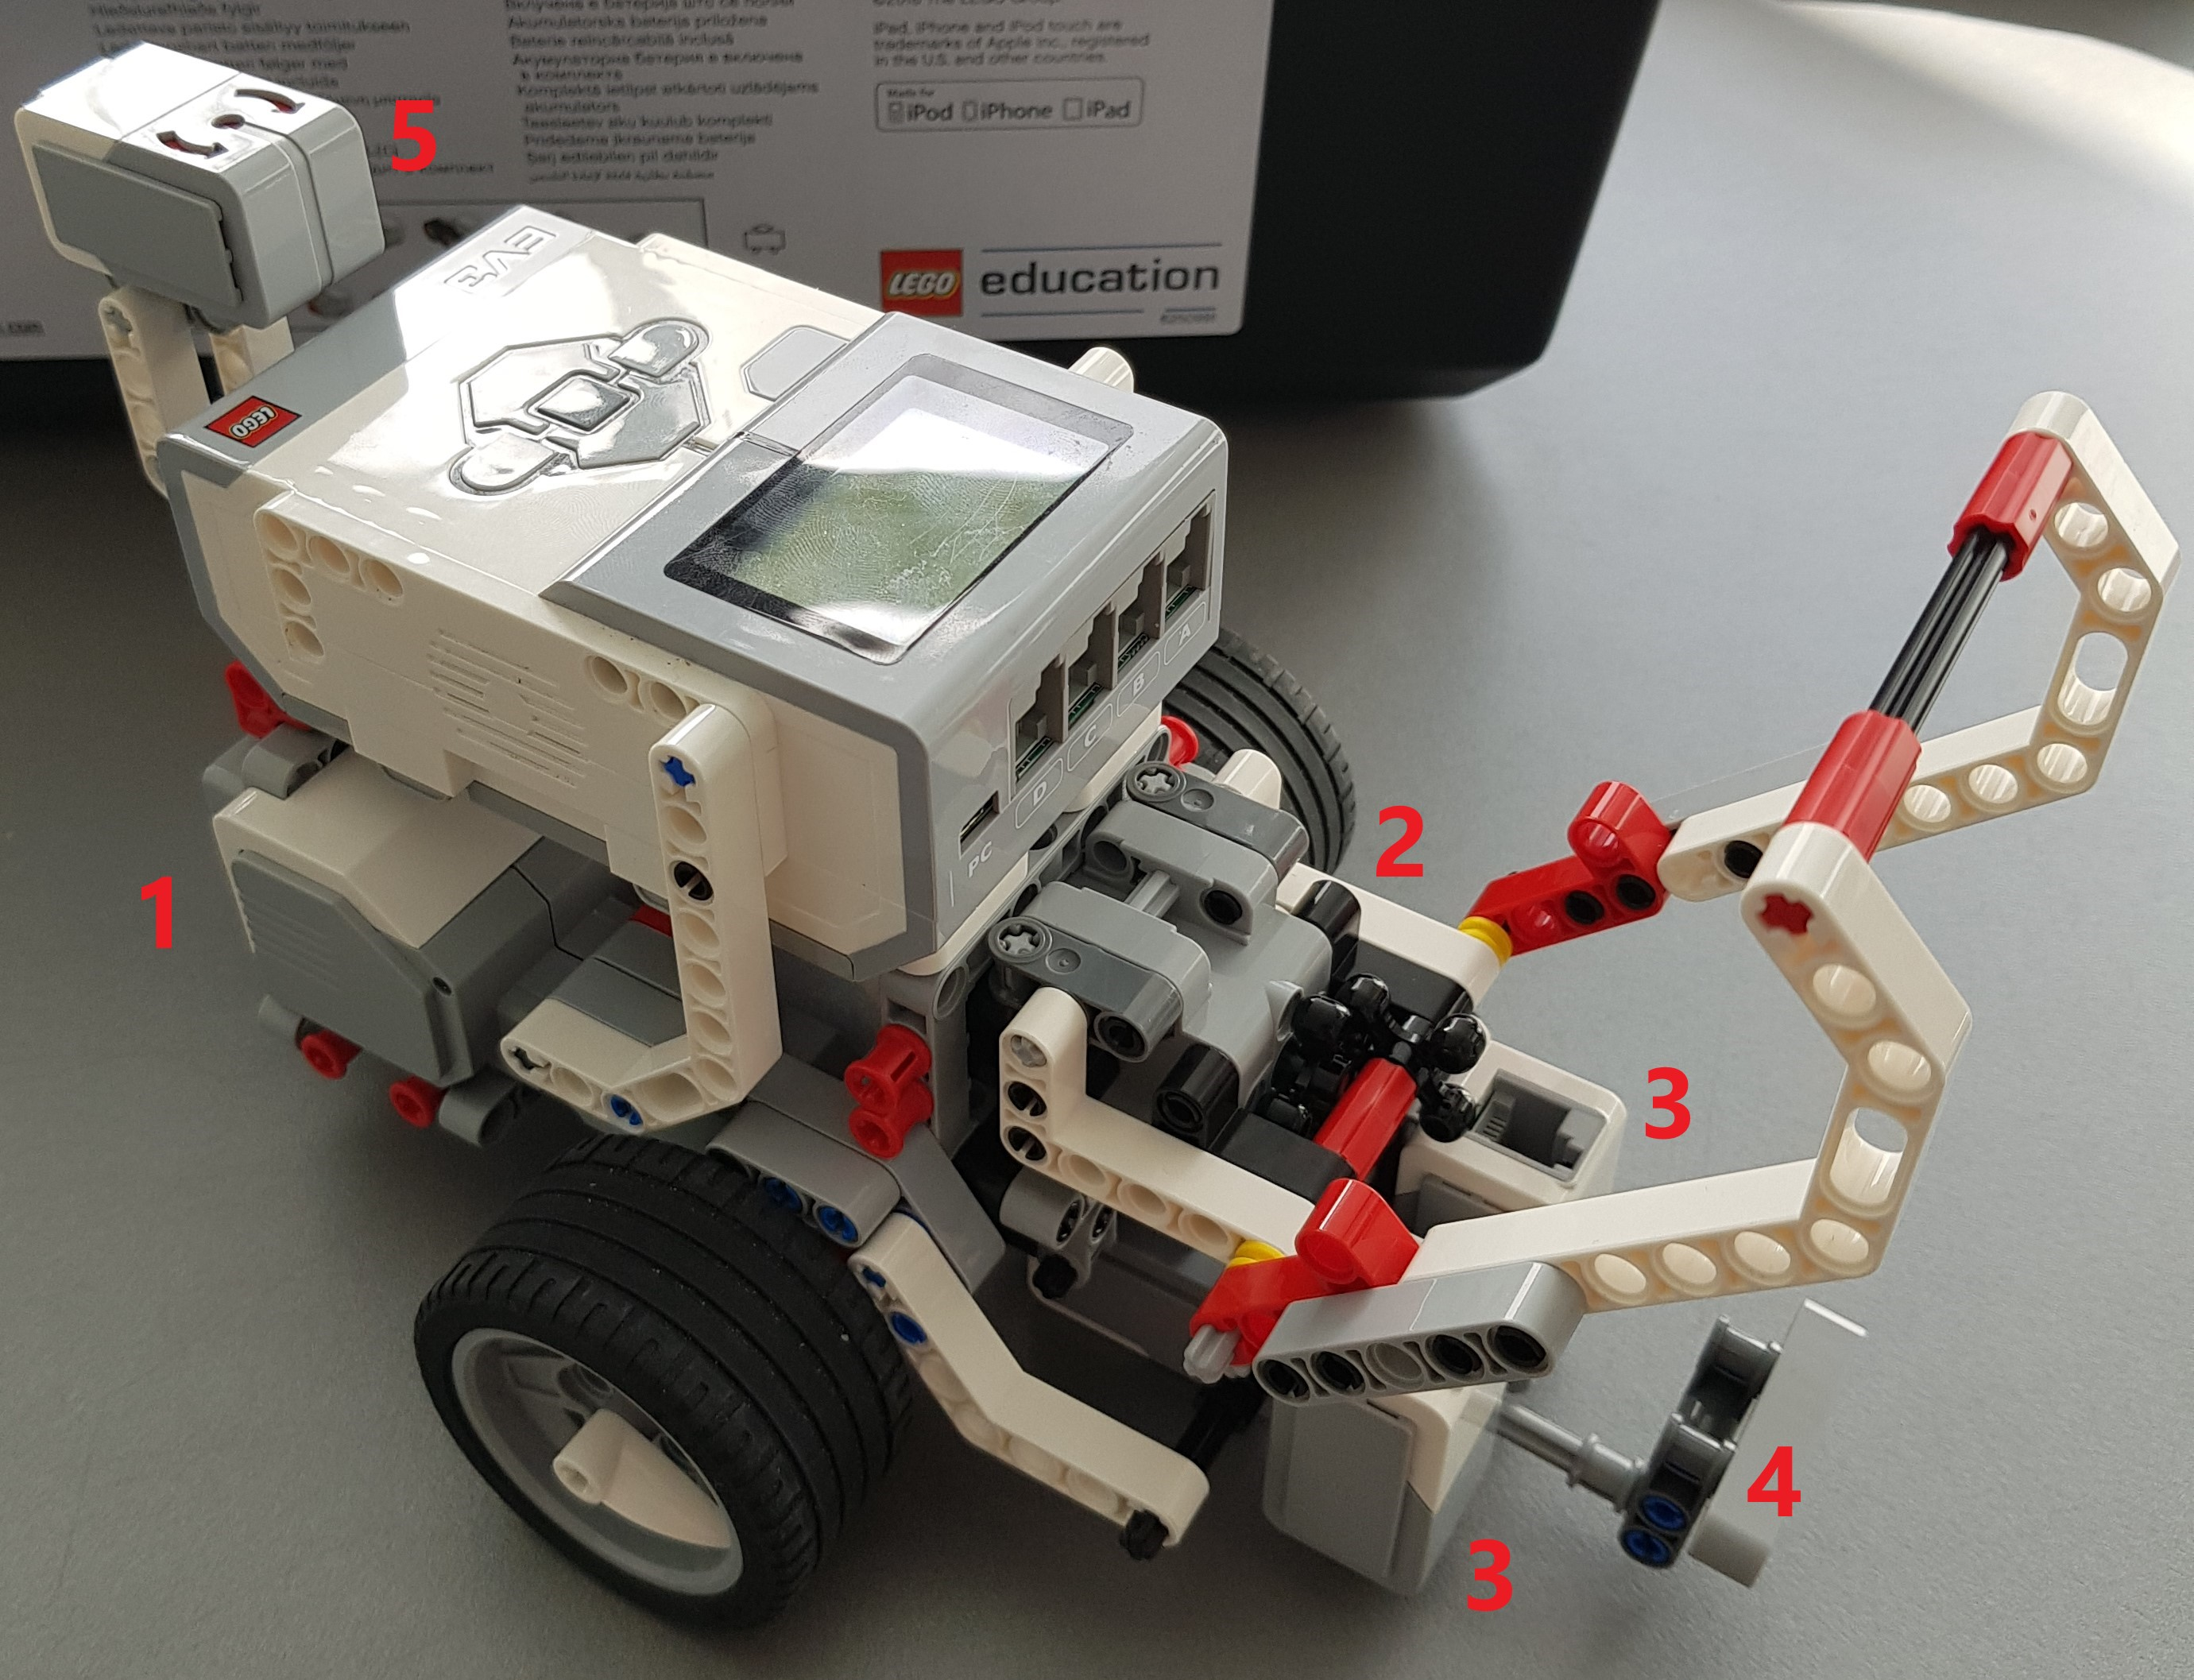
\includegraphics[width=0.8\textwidth]{figures/old_robot_design/robot_design_side.jpg}
        \caption{First design iteration of robot}
        \label{fig:1st_robot_design_it}
    \end{subfigure}
    \hfill
    \begin{subfigure}[t]{0.48\textwidth}
        \centering
        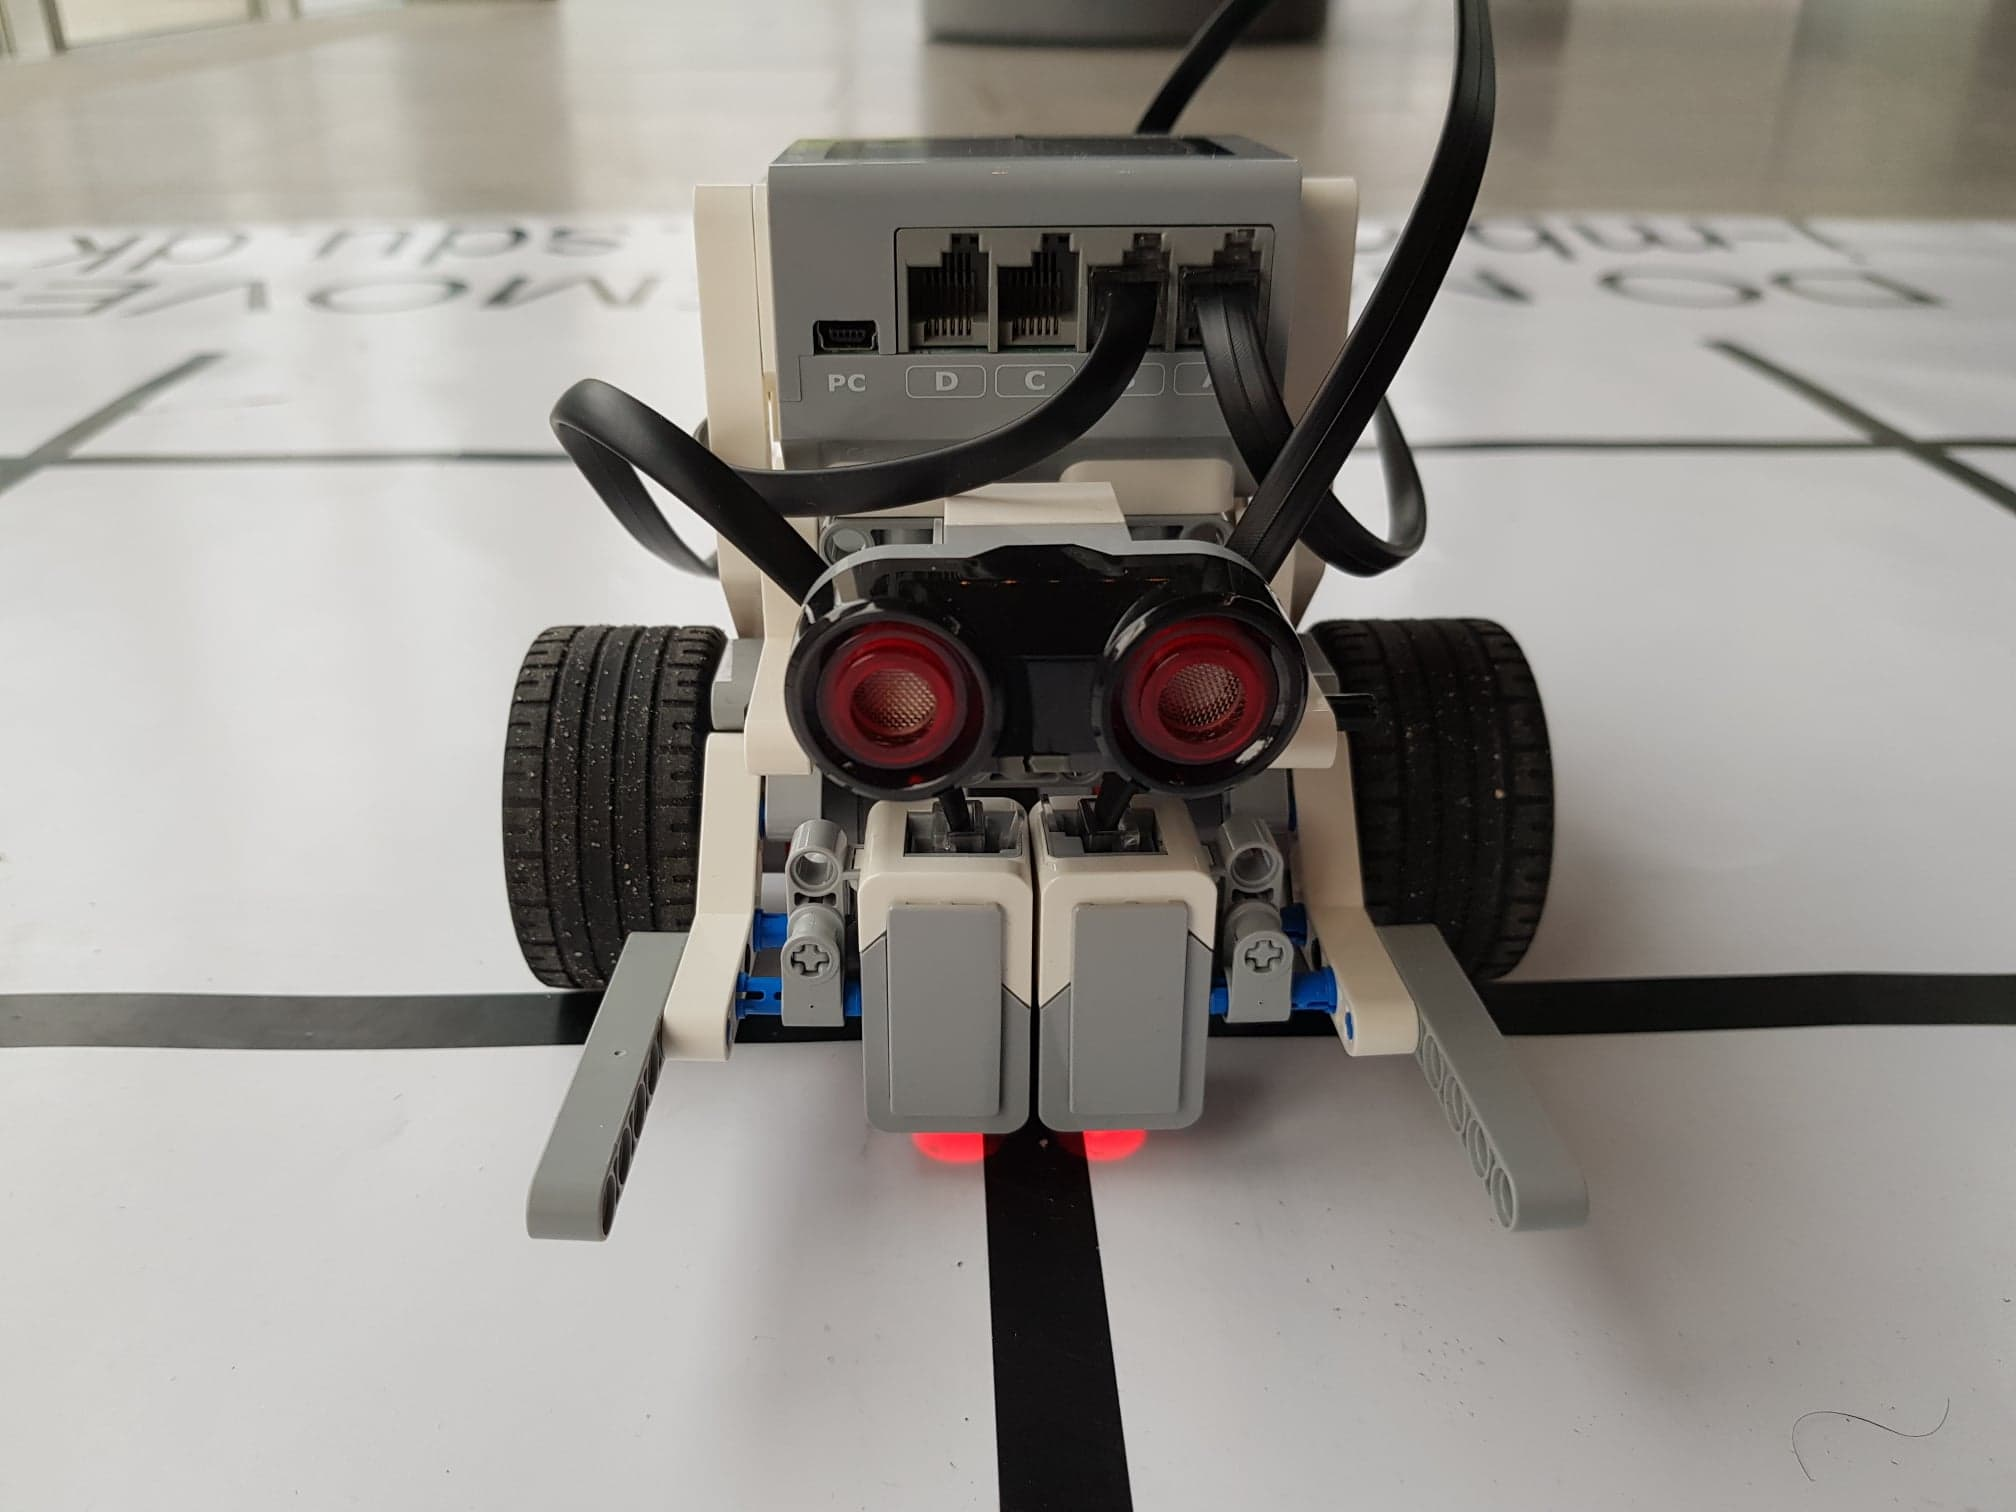
\includegraphics[width=0.8\textwidth]{figures/old_robot_design/color_sensor_linefollower.jpg}
        \caption{Second design iteration of robot}
        \label{fig:2nd_robot_design_it}
    \end{subfigure}
    \caption{First and second design iteration of the robot}
    \label{fig:1st_2nd_robot_design_it}
\end{figure}

In the first design iteration of the robot illustrated in \autoref{fig:1st_robot_design_it} it was quickly discovered many of the modules was not necessary, thus the second design iteration illustrated in \autoref{fig:2nd_robot_design_it} was only built with 2 color sensors, 2 motors, and an ultrasonic sensor. This design was used until the robot had to push the jewels. It was discovered that the jewels could slide to the sides when pushing, thus make the robot unable to catch the jewels when pushed again. Furthermore, the ultrasonic sensor was deemed unnecessary. The final design iteration of the robot is shown in \autoref{fig:final_robot_design_it}

\begin{figure}[H]
    \centering
    \begin{subfigure}[t]{0.48\textwidth}
        \centering
        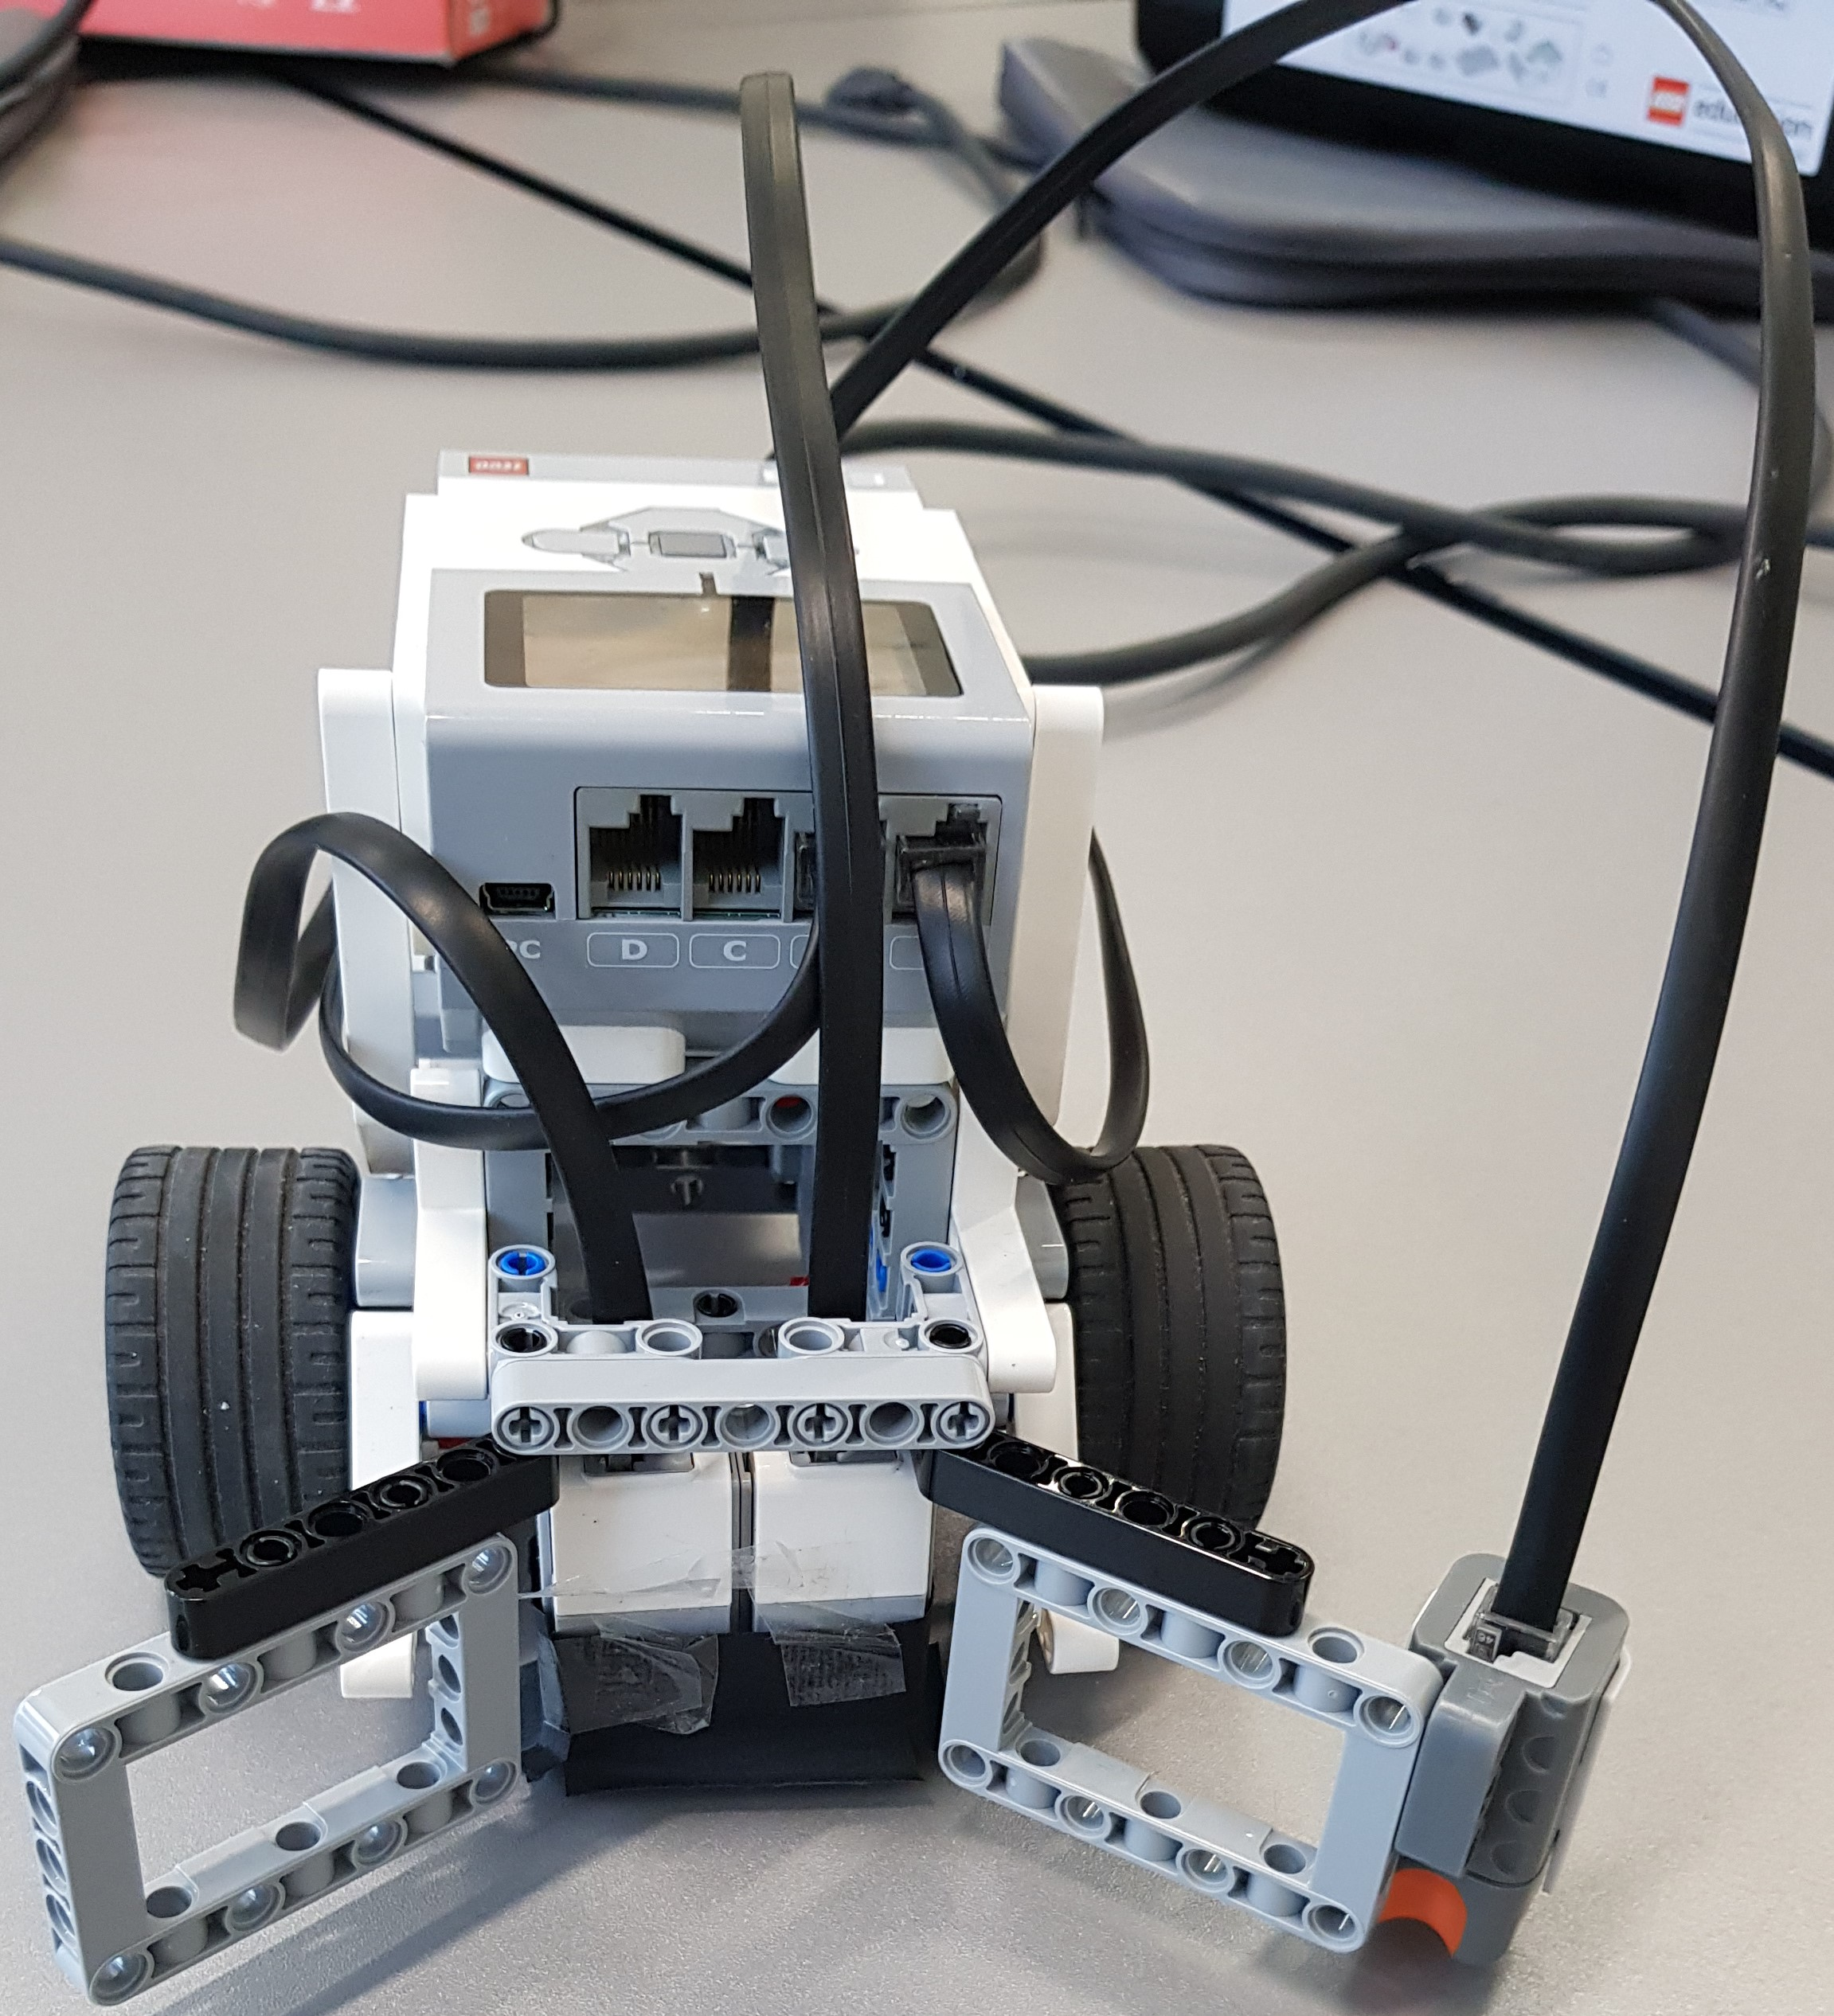
\includegraphics[width=0.68\textwidth]{figures/robot_design/final_robot_design_front.jpg}
        \caption{Final robot design front.}
        \label{fig:final_robot_design_it_front}
    \end{subfigure}
    \hfill
    \begin{subfigure}[t]{0.48\textwidth}
        \centering
        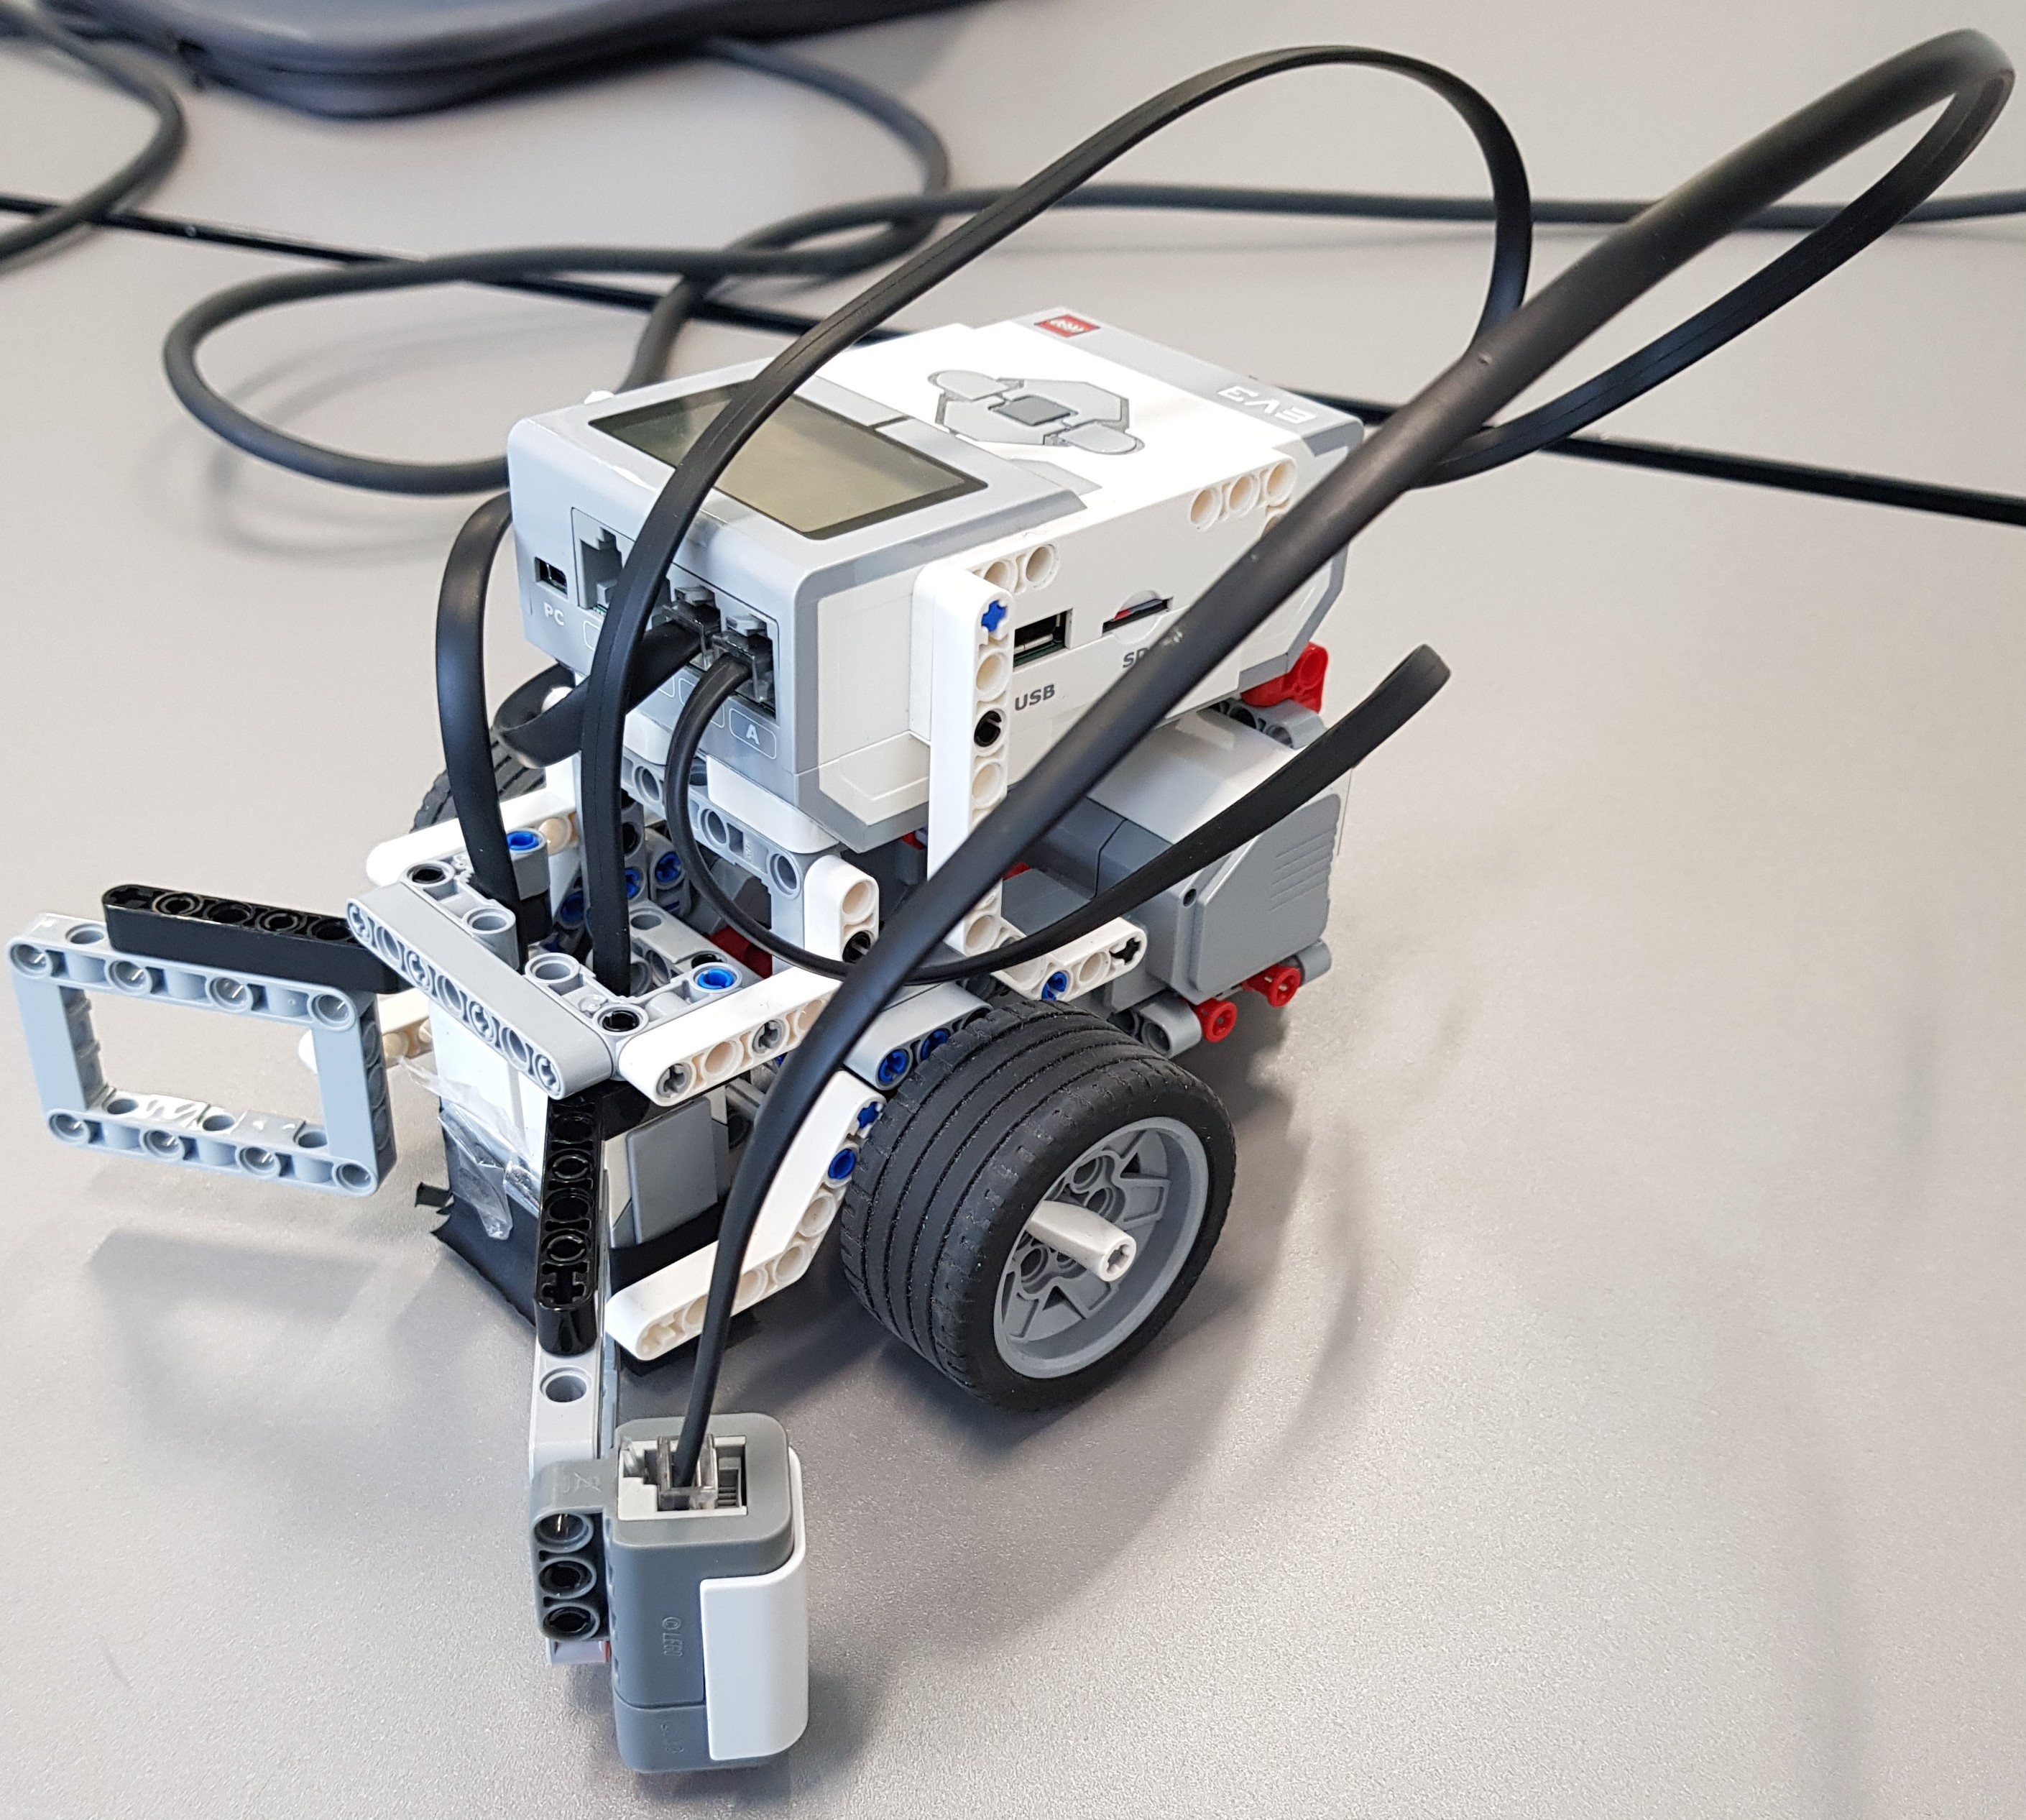
\includegraphics[width=0.8\textwidth]{figures/robot_design/final_robot_design_side.jpg}
        \caption{Final robot design side.}
        \label{fig:final_robot_design_it_side}
    \end{subfigure}
    \caption{The final robot design.}
    \label{fig:final_robot_design_it}
\end{figure}

To counteract the jewels sliding to the sides when pushing, the gripper was re-engineered to the design shown in \autoref{fig:final_robot_design_it}. Furthermore, a light sensor was added to the gripper to get more robust intersection detection, than using both color sensors. The final design of the robot consist of the following modules.
\begin{enumerate}
    \item Driving base module with EV3 microcontroller and 2 large motors
    \item Grabber module
    \item Color sensor module with 2 color sensors
    \item Light sensor module with 1 light sensor
\end{enumerate}

\subsection{Controlling the Robot} \label{subsec:controlling}
The design of the control system for the robot will be described in this section.

A behavior-based control system divides the overall problem into behaviors, where each behavior is responsible to solve the task correctly. In contrast to classical robot control where a central controller controls the whole system and normally is advanced and difficult to modify, behavior-based systems are easy to modify and have a fast prototype pipeline. Thus, the control of the LEGO Mindstorm robot is done as a behavior-based system. 

\subsubsection{Behaviors} \label{subsubsec:behaviors}
The behaviors in behavior-based systems can be interconnected with each other to either overrule one behavior from another or to give inputs to a behavior to modify it. All the behaviors used to solve the Sokoban puzzle is shown in table \ref{tab:behaviours}. 

\begin{table}[H]
\centering
\resizebox{0.6\textwidth}{!}{%
\begin{tabular}{lll}
\toprule
\textbf{Number} & \textbf{Name} & \textbf{Description} \\ \midrule
1 & Follow & Follow a line. \\
2 & Intersection & Detect an intersection. \\
3 & Forward & Run forward for a certain period. \\
4 & Backwards & Run backwards for a certain period. \\
5 & Turn left & Rotate left for a certain period. \\
6 & Turn right & Rotate right for a certain period. \\
7 & Turn $180$ & Rotate $180$ degrees. \\ \bottomrule
\end{tabular}
}
\caption{Berhaviours of the robot to solve the sokoban puzzle.}
\label{tab:behaviours}
\end{table}

\textbf{Follow:} The following behavior is used to keep the robot onto the line of the Sokoban map. The behavior is designed as a reactive controller, by taking the two color sensors outputs and using the outputs to set speed on the wheels. The left color sensor output is used to control the left motor and the right color sensor output is used to control the right motor. Thus, making a controller that is "scared" of black lines. The color sensor's values are scaled with a constant to control the speed of the robot.

\textbf{Intersection:} The intersection behavior controls whether an intersection has been detected or not. This is done by using the light sensor output. When the light intensity is lower than a specific threshold an intersection is present.

\textbf{Forward:} The forward behavior sets both wheels to a constant positive velocity in a specific time interval. The behavior is used to drive over intersections.

\textbf{Backwards:} The Backwards behavior sets both wheels to a constant negative velocity in a specific time interval. The behavior is used to reverse the robot away from a jewel after placing it.  

\textbf{Turn left:} The turn left behavior starts by driving forward over the intersection in order to make a $90$ degree left turn afterward.

\textbf{Turn right:} The turn right behavior starts by driving forward over the intersection in order to make a $90$ degree right turn afterward.

\textbf{Turn 180:} The turn $180$ behavior is used to turn $180$ degrees after reversing away from the jewel, in order to position the robot correctly after a jewel push. 

\subsubsection{Decision rules for switching behavior}
For the robot to solve the real-life Sokoban puzzle using the behaviors described above, decision rules are designed in order to execute the correct behavior. The decision rules implemented on the robot decide which behavior to execute based on a current action. The current action is from a sequence of actions generated beforehand by the path planner, which is described in \autoref{sec:solver}. A flow chart of the decision rules is shown in \autoref{fig:decision_rules}.

\begin{figure}[H]
    \centering
    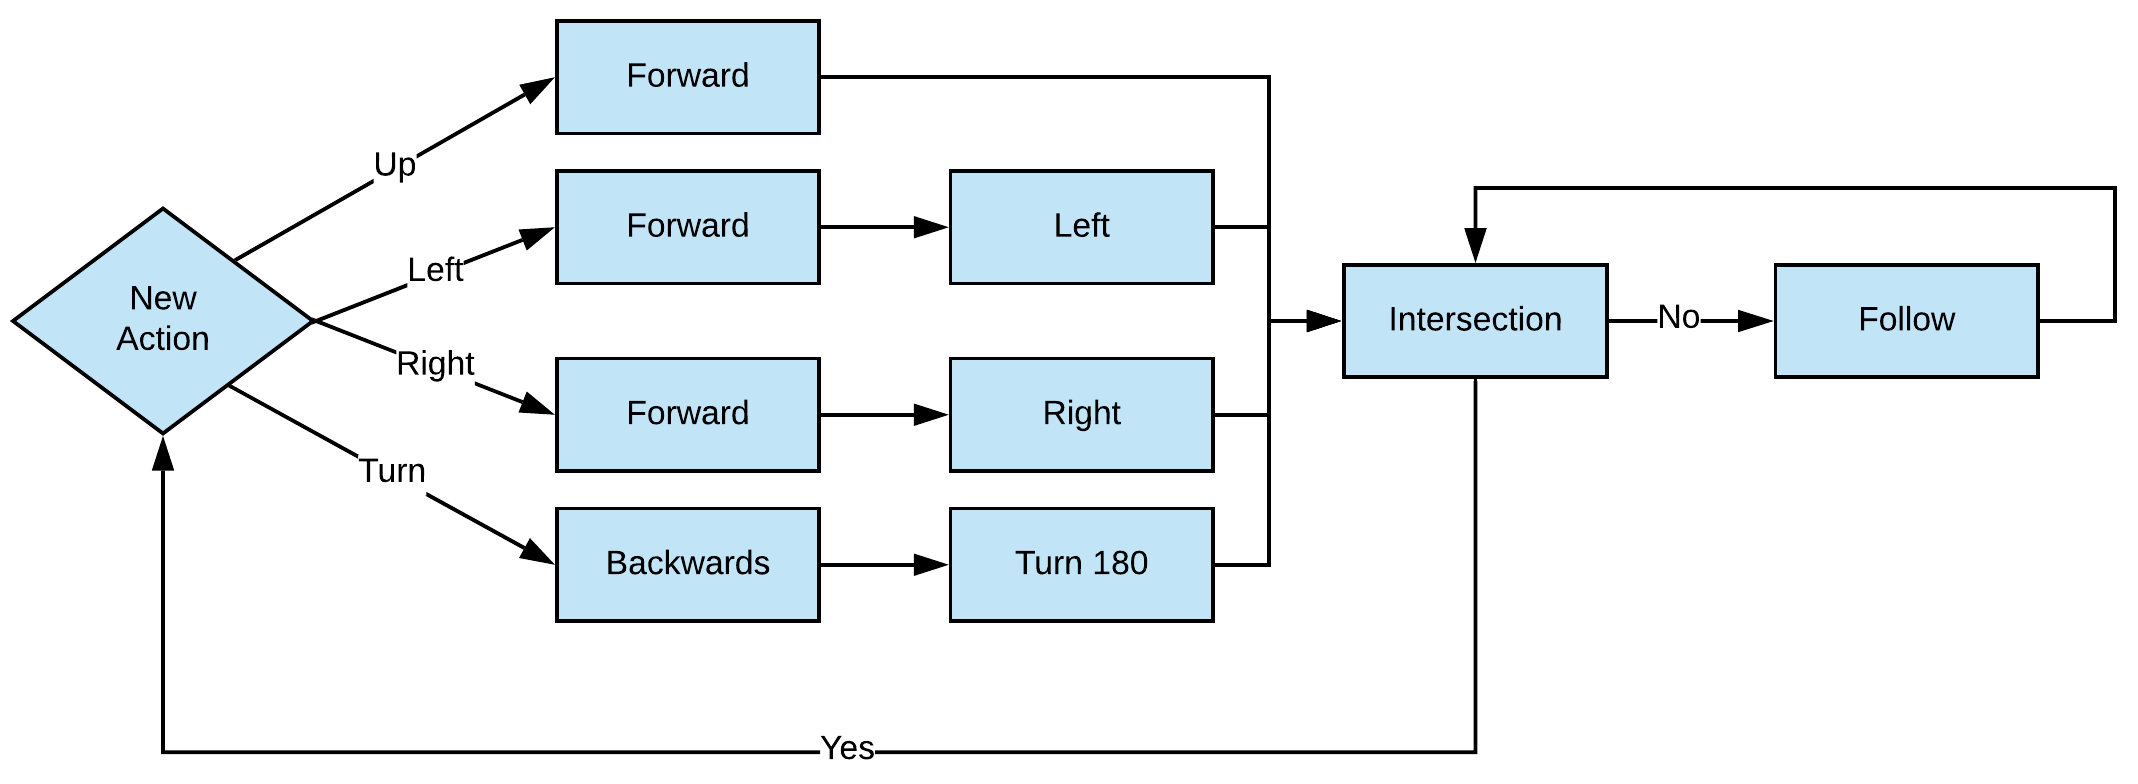
\includegraphics[width=1\columnwidth]{figures/robot_design/Decision_rules_behaviors.png}
    \caption{Flow chart of decision rules for executing behaviors. Diamond is function, Square is behavior. If there is no text on an arrow the condition is: behavior done executing.}
    \label{fig:decision_rules}
\end{figure}

\subsection{Performance Evaluation of the Final Robot Design}\label{subsec:robot_eval}
In this section the performance of the final robot design is tested. Each test was conducted with three different color sensor scaling factors $1$, $1.25$, $1.5$. The lower the color sensor scale the higher the speed of the robot. The following tests are conducted.

\textbf{180 degree turns in a straight line:}  
The robot was set to drive forward one time followed by a backward and $180$ degree turn. This sequence was repeated 10 times, counting as one try. The robot did 10 tries. 

\textbf{Left and Right turns in a circle:}
The robot was set to drive around in a circle of 10 laps. The test was conducted 10 times each for right and left turns. 

\textbf{Intersection detection:} 
The robot was set to drive up to the nearest intersection with the behavior follow. When detecting an intersection it drove backward and then repeated the sequence. This was done 10 times counting as one try. The robot did 10 tries. 

\textbf{Final map:}
The last test conducted was the robot running the optimal solution for the final map. The final map is illustrated in \autoref{subfig:map5}. The solution was found by the algorithm described in \autoref{sec:solver}. The robot only ran the solution once for every color sensor scaling.

All of the test described above is illustrated as GIFS and can be seen on \cite{code} in the README.md file. 

\textbf{Results:}\\
From the results of all the turning test in \autoref{tab:turn_test}, it can be seen that the robot is robust when turning right or left and when detecting intersections because zero failure were observed. However, when looking at the $180$ degree turn test it can be seen that the color sensor scaling has a big impact on repeatability. When the $180$ degree turn test was conducted it was observed that the primary reason for failure was because the robot was located skew relative to an intersection right before a turn. This meant the robot overshot when turning because the turning is a hardcoded value. 

% \begin{table}[H]
% \centering
% \resizebox{\textwidth}{!}{%
% \begin{tabular}{l|l|l|l}
%  & \textbf{$180$ Degree turn} & \textbf{Right turn} & \textbf{Left turn} \\ \hline
% Color sensor scaling & \begin{tabular}[c]{@{}l@{}}Mean number of rounds\\ before failure\end{tabular} & \begin{tabular}[c]{@{}l@{}}Mean number of rounds\\ before failure\end{tabular} & \begin{tabular}[c]{@{}l@{}}Mean number of rounds\\ before failure\end{tabular} \\ \hline
% $1$ & $4$ & $10$ & $10$ \\
% $1.25$ & $5.3$ & $10$ & $10$ \\
% $1.5$ & $9$ & $10$ & $10$
% \end{tabular}
% }
% \caption{Results for all the turning tests}
% \label{tab:turn_test}
% \end{table}

\begin{table}[H]
\centering
\resizebox{\textwidth}{!}{%
\begin{tabular}{l|l|l|l|l}
\toprule
 & \textbf{180 Degree turn} & \textbf{Right turn} & \textbf{Left turn} & \textbf{\begin{tabular}[c]{@{}l@{}}Intersection \\ detections\end{tabular}} \\ \hline
Colorsensor Scaling & \begin{tabular}[c]{@{}l@{}}Mean number of rounds\\ before failure\end{tabular} & \begin{tabular}[c]{@{}l@{}}Mean number of rounds\\ before failure\end{tabular} & \multicolumn{1}{l|}{\begin{tabular}[c]{@{}l@{}}Mean number of rounds\\ before failure\end{tabular}} & \begin{tabular}[c]{@{}l@{}}Mean number of rounds\\ before failure\end{tabular} \\ \hline
1 & 4 & 10 & \multicolumn{1}{l|}{10} & 10 \\
1.25 & 5.3 & 10 & \multicolumn{1}{l|}{10} & 10 \\
1.5 & 9 & 10 & \multicolumn{1}{l|}{10} & 10 \\ \bottomrule
\end{tabular}
}
\caption{Results for all the turning tests and the intersection test.}
\label{tab:turn_test}
\end{table} 

The results of the final map test is shown in \autoref{tab:final_map_test}. From the results, it can be seen that a lesser color sensor scaling value corresponds to a quicker time. However, when conducting the test it was observed that the robot was more unstable running at a lower color sensor scaling. Thus, if the test was to be run multiple times, the failure rate of the robot may yield to be higher with a lower color sensor scaling. 

\begin{table}[H]
\centering
\begin{tabular}{l|l}
\toprule
\textbf{Color sensor scaling} & \textbf{Time {[}Minuts{]}} \\ \hline
1 & 5 \\
1.25 & 6.1 \\
1.5 & 6.42 \\ \bottomrule
\end{tabular}
\caption{The total time for completing the final map with corresponding color sensor scaling.}
\label{tab:final_map_test}
\end{table}

\end{document}